\documentclass[a4paper,10pt]{article}

\author{Santiago Domínguez Collado}
\title{Borrador TFG}

\usepackage{lmodern}
\usepackage[T1]{fontenc}
\usepackage[spanish]{babel}
\usepackage[utf8]{inputenc}
\usepackage{mathtools}
\usepackage{ amssymb }
\usepackage{graphicx}
\usepackage[margin=1.50in]{geometry}
\graphicspath{{imagenes/}}
\usepackage{float}
\usepackage{listings}
\usepackage{float}
\usepackage[none]{hyphenat} %no corta las palabras al compilar el documento
\sloppy %como no se cortan las palabras el texto se descuadra, justifica los p�rrafos
\usepackage{geometry}
\geometry{textwidth=474pt} %Corrige algo de geometry
\begin{document}
\begin{center}
\begin{LARGE}
Machine Learning \\
\vspace*{0.15in}
\UseRawInputEncoding
Borrador TFG
\end{LARGE}
\end{center}
\begin{center}
\begin{large}
Santiago Domínguez
\end{large}
\end{center}

\section{Base matemática del Machine Learning.}
\label{}

El estudio de optimización se lleva a cabo con el objetivo de maximizar o minimizar una función \textit{f}.
Por ejemplo, en nuestro caso, minimizar la función de error implica hallar los parámetros que la definen, cuando en los valores de estos la función alcanza su mínimo.
Nos serviremos de la teoría de la optimización para alcanzar los valores en los que la función alcanza su mínimo absoluto. Estos valores son referidos como parámetros óptimos.
\subsection{Teorema de Weierstrass.}

El teorema de Weierstrass establece que en toda función continua \textit{f}, alojada en un intervalo cerrado y acotado, dicha función alcanza sus valores máximos y mínimos en puntos del intervalo.
 \[Si \hspace{0.20cm} \textit{f} \in C(A) \Rightarrow \exists x_{1},x_{2} \in A \mid f(x_{0}) \leq f(x) \leq f(x_{1}) \hspace{0.20cm} \forall x \in A\] 
\textbf{Definición 1.1. (Condición necesaria de extremo.)}
\noindent
\[Sea \hspace{0.20cm} \vec{x} \in \mathring{A}, y\hspace{0.20cm} \textit{f}\hspace{0.20cm} derivable\hspace{0.20cm} en \hspace{0.20cm}x \Rightarrow \nabla f(\vec{x}) = (0,...,0)\]
\textbf{Demostración:} \[f \text{derivable en x } \Rightarrow f(\vec{x}+tei)=\textit{g(t)}\Rightarrow \] 
\[ \Rightarrow \text{g'} (0)=0= <\text{ei,} \nabla f(\vec{x}) >\] 
\[\text{ Siendo }  \nabla f(\vec{x})= \frac{\partial f}{\partial xi} \partial xi (\vec{x})\]
La condición anterior no es suficiente, puesto que:
\begin{itemize}
    \item Puede ocurrir que $\nabla f(A) = 0$ y sea punto de silla.
    \item Puede ser el extremo relativo.
\end{itemize}
\subsection{Búsqueda de mínimo absoluto.}

Debemos buscar un máximo o mínimo en el conjunto interior $\mathring{A}$, empezando por los puntos en la frontera del conjunto, después los puntos sin derivada y por último los puntos con derivada nula. Existen condiciones para comprobar si cada punto con derivada nula es o no máximo o mínimo. Con matriz M y vector $\vec{x}$:
\begin{itemize}
\item M es definida positiva $\Longleftrightarrow x^TMx \geq 0$y$x^TMx=0\Leftrightarrow x=0$
\item M es definida negativa  $\Longleftrightarrow x^TMx \leq0$y$x^TMx=0\Leftrightarrow x=0$
\item M es semidefinida positiva  $\Longleftrightarrow x^TMx \geq0$y$x^TMx\neq0\Leftrightarrow x=0$
\item M es semidefinida negativa  $\Longleftrightarrow x^TMx \leq0$y$x^TMx\neq0\Leftrightarrow x=0$
\end{itemize}
\textbf{Definición 1.2. (Matriz Hessiana.)}
Sea \textit{f}, se dice matriz hessiana a la matriz tal que, $\textit{D} \subseteq R \rightarrow R^2$, \textit{A} un punto perteneciente al conjunto \textit{D}, tal que \textit{f} es diferenciable dos veces en el punto \textit{A}.
\[
\begin{vmatrix}\textit{H(A)}\end{vmatrix}=
\begin{vmatrix}
    f_{xx} & f_{xy} \\
    f_{yx} & f_{yy}
\end{vmatrix}
\]
\textbf{Teorema 1.1. (Clasificación de extremos mediante matriz hessiana.)}
Sea \textit{f}, $\textit{D} \subseteq R \rightarrow R^2$, \textit{D}  un conjunto abierto, con derivadas segundas continuas en un entorno de \textit{A} punto críticos de \textit{f}. Y considerando $\begin{vmatrix}\textit{H(A)}\end{vmatrix}$ como el determinante de la matriz hessiana en el punto \textit{A}:
\begin{itemize}
    \item Si $\begin{vmatrix}\textit{H(A)}\end{vmatrix}>0$ y $ f_{xx}(A)>0$, entoces \textit{f} tiene un mínimo realtivo en \textit{A}.
    \item Si $\begin{vmatrix}\textit{H(A)}\end{vmatrix}>0$ y $ f_{xx}(A)<0$, entoces \textit{f} tiene un máximo realtivo en \textit{A}.
    \item Si $\begin{vmatrix}\textit{H(A)}\end{vmatrix}<0$, entoces \textit{f} tiene un punto de silla en \textit{A}.
    \item Si $\begin{vmatrix}\textit{H(A)}\end{vmatrix}=0$, entoces no podemos sacar conclusiones.
\end{itemize}


\subsection{Convexidad.}

El estudio de la convexidad permite afirmar que un mínimos relativo es absoluto, por lo tanto, nos interesa demostrar la convexidad de la función de error para determinar nuestro prámetros óptimos.

\begin{itemize}
\item El dominio es cerrado y acotado: gradualmente expresado con restricciones de desigualdad. Algoritmo de Karush-Khun-Tucker.
\item Hay restricciones de igualdad: Algoritmo de multiplicadores de Lagrange.
\item En dominios convexos.
\end{itemize}
\textbf{Definición 1.3.} 
\[x_{L} \rightarrow \text{mínimo local. Si } exists x_{1} |  f(x_{1}) < f(x_{L})\]
\[f(x_{L})\leq f(tx_{L})+(1-t)x_{1}\leq tf(x_{L})+(1-t)f(x_{1})<f(x_{1})\]
\textbf{Definición 1.4.}
$\textit{f}: \textit{A}\rightarrow (R)$, \textit{f} es convexa en $x_{0}$ si lo es en un entorno de $x_{0}$. En tal caso, \textit{Hf($x_{0}$)} es definida positiva.
\subsection{Regresión Lineal}

Sea un conjunto de datos $(xi,yi)^n_{i=1}$, queremos obtener la recta  que mejor se ajuste a la hipótesis $h\theta(x)= ax+b$ (puede tener  más parámetros). Para ello, hallamos los parámetros de h$\theta$  minimizando la función del error cuadrático medio.

\[ \text{i.e. escoger (a,b)} \in R^2 | \text{ EMC} = \frac{1}{N} \sum_{i=1}^{N}(y_{i}-ax_{i}-b)^2 \text{mínimo.} \]
\subsection{Mínimos y máximos locales:}
\[\frac{\partial{H}}{\partial{b}}=-2\sum_{i=1}^{N}y_{i}-ax_{i}-b=0\Rightarrow \sum_{i=1}^{N}ax_{i}+bN=\sum_{i=1}^{N}y_{i}\Rightarrow b=\Bar{y}-a\Bar{x}\]
\[\frac{\partial{H}}{\partial{a}}=-2\sum_{i=1}^{N}(y_{i}-ax_{i}-b)x_{i}=0\Rightarrow \sum_{i=1}^{N}x_{i}y_{i}=a\sum_{i=1}^{N}x_{i}^2+b\sum_{i=1}^{N}x_{i}\Rightarrow a \frac{1}{N}\sum_{i=1}^{N}x_{i}^2+(\Bar{y}-a\Bar{x})\Bar{x}=\sum_{i=1}^{N}x_{i}y_{i}\Rightarrow\] 
\[\Rightarrow a[ \,\frac{1}{N} \sum_{i=1}^{N} x_{i}^2-\Bar{x}^2] \,+\Bar{y}\Bar{x}=\frac{1}{N}\sum_{i=1}^{N}x_{i}y_{i}\Rightarrow a\partial_x^2=s_{xy}\Rightarrow\]
\[\boxed{a=\frac{s_{xy}}{\partial_{x^2}}, b=\Bar{y}-\frac{s_{xy}}{\partial_{x^2}}\Bar{x}}\]
$\Rightarrow$ e.d. un único extremo local.\\
\\
Hessian de H: $
\begin{bmatrix}
    \frac{\partial^2 H}{\partial a^2} & \frac{\partial^2 H}{\partial a \partial b} \\
    \frac{\partial^2 H}{\partial a \partial b} & \frac{\partial^2 H}{\partial a^2}
\end{bmatrix} \Rightarrow 4(N\sum_{i=1}^{N}x_{i}^2-(\sum_{i=1}^{N}x_{i})^2)\geq 0 \Leftrightarrow \frac{1}{N}\sum_{i=1}^{N}x_{i}^2 - \Bar{x}^2 \geq 0 \Rightarrow$ \textit{f} es convexa \\ y el mínimo local es global.

\subsection{Regresión lineal multivariable.}

El estudio regresión lineal multivariable se utiliza para hallar la relación entre múltiples variables con su salida, con el objetivo de formular una hipótesis que será útil para predecir futuros resultados con nuevas entradas. Supongamos que tenemos las siguientes entradas y salidas: 

\begin{figure}[H]
\centering
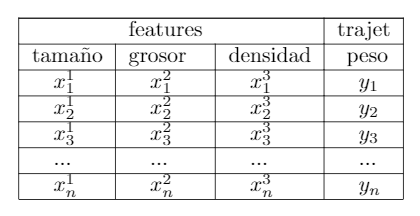
\includegraphics[scale=0.8]{Annotation 2020-03-23 133547}
\end{figure}
 \[\text{Hiperespacio } H(a_{1},a_{2},a_{3},a_{4})=\frac{1}{N}\sum_{i=1}^{N}(a_{1}x_i^1+a_{2}x_i^1+a_{3}x_i^1+a_{4}-y_{i})^2 \text{¿ Es } \vec{a}\text{ minimizante?}
\]
\[H:R^4\rightarrow R \begin{bmatrix}
    x_{1}^1 & x_{1}^2 & x_{1}^3 & x_{1}^4 1 \\
    .&.&.&.\\
    .&.&.&.\\
    .&.&.&.\\
    x_{N}^1 & x_{N}^2 & x_{N}^3 & x_{N}^4 1
\end{bmatrix} \in M_{M*n}. \hspace{0.20cm} y=\begin{bmatrix}y_{1}\\y_{2}\\.\\.\\.\\y_{N}\end{bmatrix}\] \\ \[H(\vec{a},b)=||X\vec{a}-y||^2 = <x\vec{a}-\vec{y},x\vec{a}-y>=<x\vec{a},x\vec{a}>-2<X\vec{a},y>+<y,y>\]
\[\nabla H(a)=\nabla<x\vec{a},x\vec{a}>-2\nabla<x\vec{a},\vec{y}>=0\Leftrightarrow \boxed{ \vec{a}=(X^T X)^{-1} X^T y}\]

\subsection{Método directo.}

El anterior método explicado en el apartado de regresión lineal multivariable muestra cómo obtener la hipótesis de forma directa, analítica, no obstante en la realidad, el cálculo de la inversa de una matriz se evita en la mayoría de las ocasiones debido a la complejidad que esta requiere O($n^3$).\\
En su lugar, métodos iterativos como steepest descent, el cual “desciende” por la función de error gracias al cálculo constante de los parámetros en cada iteración, muestran una complejidad inferior O(n2), la cual es viable computacionalmente para trabajar. 

\subsection{Regresión polinomial.}

Cuando nuestro modelo no se ajusta a una linea recta, la Regresión Lineal no nos sirve para definir una hipótesis que se ajuste a nuestro modelo de datos.
IMAGEN DE GRÁFICA 1
La solución más tentaiva que se plantea para aborar este dataset es añadir un nuevo parámetro a nuestra hipótesis que multiplique a la variable ya presente, pero esta vez, elevada a un factor mayor. 
\[
 y=\theta_0+\theta_1 x+\theta_2 x^2
\]
\[
 min\sum_{i=1}^{N}(y-\theta_0-\theta_1 x-\theta_2 x^2)^2\longrightarrow \hat{\theta_0},\hat{\theta_1},\hat{\theta_2} \Rightarrow \text{esto ha funcionado. GRÁFICA 1 CON UNA CURVA DECENTE}
\] 
Si consideraramos una hipótesis más ambiciosa como $y=\theta_0+\theta_1 x+\theta_2 x^2 ...\hspace{0.15cm} \theta_20 x^n$ pero esto nos llevaría a un ajuste de nuestro modelo demasiado preciso como para funcionar correctamente con datos de testeo. Esto se conoce como \textit{Overfitting} o \textit{Variance problem}.
\\Eso nos lleva al problema de determinar el número de parámetros del modelo. Es decir, necesitamos saber cómo aplicar regresión polinomial.
\subsection{Aplicación de regresión polinomial.}

En la práctica, la decisión de aplicar regresión lineal o polinomial puede no ser algo trivial, por ello, antes de reflexionar sobre el número de parámetros que queremos aplicar a nuestro modelo, debemos primero, determinar si la naturaleza del problema corresponde a un problema polinomial, o si por el contrario, la regresión lineal es suficiente para abordarlo.
\subsubsection{Coeficiente de Pearson.}

El coeficiente de correlación lineal de Pearson ($r_xy$) nos sirve para determiar la naturaleza de la relación que guardan los datos entre sí, si es coeficiente es cercano a 1 ó -1, esto indica que no es necesario aplicar regresión polinomial.
\[
r_{xy}=\frac{s_{xy}}{s_x s_y}
\]
El coeficiente de Pearson es válido solo cuando se cumplan las siguientes condiciones:
\begin{itemize}
    \item Los datos sean muestras independientes, es decir, no haya auto-correlación entre ellos.
    \item Los datos presenten una distrubución normal.
    \item Homocedaesticida (pone en internet que esto es en los modelos, preguntar a iván)
\end{itemize}
\subsubsection{Coeficiente de Spearman.}

El coeficiente de Spearman ($\rho$) es una medida de correlación utilizada en lugar del coeficiente de Pearson, cuando no se cumple algunas de las condiciones mencionadas en el apartado anterior. el resultado de este se interpreta al igual que en el coeficiente de Pearson, si el resultado es ceacano 1 ó -1, no es necesario aplicar regresión polinomial.
\[
\rho = 1 - \frac{6\sum D^2}{N(N^2 - 1)}
\]
Siendo D la diferencia entre los correspondientes estadísticos de orden de x - y, y siendo N el número de datos.
\subsubsection{Determinación del número de parámetros.}

Partiendo del supuesto de que los datos de nuestro problema presenten una clara necesidad de ser abordados por regresión polinomial, El siguiente paso para definir el modelo será encontrar un número de parámetros que se ajuste bien a los datos sin presentar overffiting, o por el contrario underffiting, el cual se dice cuando nuestra curva presenta un vago ajuste los datos. 
\[
Error (x) = (E[\hat{f}(x)]-f(x)^2+E[(\hat{f}(x)-E[\hat{f}(x)])^2]+\sigma^2_irr (\text{error irreducible})
\]
\subsubsection{¿Es realmente esto polinomial?}

\[
y=\theta_0+\theta_{1}x+\theta_{2}x^2
\]
Realmente la distinción entre regresión multivariable y polinomial puede verse reducida a un mero formalismo cuando consideramos que la nueva parte de la hipótesis no es más que una nueva variable de entrada en nuestro problema, variable la cual es completamente dependiente de al menos una de las variables anteriores.
\subsection{Regularización.}
\noindent
Durante el desarrollo de nuestro modelo, aplicando la teoría explicada hasta ahora, nos surge la duda de cuál es el grado que mejor resultado nos dará, o dicho de otra forma; ¿Qué grado en nuestro modelo es el que mejor se ajusta a nuestras necesidades y evita los problemas de bias y variance?\\
La regularización es la respuesta, se define regularización como la técnica que penaliza los términos de mayor gardo de nuestro modelo, permitiendonos así utilizar hipótesis de un grado considerable, por lo que no hay lugar a que aparezca el problema de bias, mientras que eludimos el problema de variance. Por ejemplo, en una hipótesis que con grado 4 nos daría variance:
\[
 y=\theta_0+\theta_1 x+\theta_2 x^2+1000\theta_3 x^3+1000\theta_4 x^4 = h_\theta (x)
\]

El anterior ejemplo nos sirve para el caso en el que sabemos qué es lo que hay que penalizar, pero para poder usarlo en un caso general, en el que no conozcamos a priori los elemento a penalizar en nuestra hipótesis, la función de costes utilizada hasta ahora será modificada:

\[
J(\vec{\theta})=\frac{1}{2m}\left[\sum_{i=1}^{m} \left(h_\theta (x^{(i)})-y^{(i)}\right)-\lambda \sum_{j=1}^{n}\theta_{j}^2\right]
\]
Como vemos, aparece la variable lambda, la cual será definida de forma empírica, una lambda muy superior a 1, provocaría variance, y si es muy cercana a 0, provocaría bias. Los valores típicos suele rondar el 0,95.\\
Además de ser una manera eficar para mejorar nuestro modelo, previniendo dos de los problemas más comunes en el desarrollo del aprendizaje automático, la implementación será tan sencilla como modificar nuestro algoritmo de aprendizaje, modificando todos los términos a partir de $\theta_0$ \\
\[
\frac{J(\theta)}{\partial\theta_j} = \frac{1}{m} \sum_{i=1}^{m} \left(h_\theta (x^{(i)})-y^{(i)}\right) x_{j}^{(i)}-\frac{\lambda}{m} \theta_j 
\]
\subsection{Escalamiento de variables (feature scaling).}
\noindent
Durante el planteamiento del problema a resolver mediante el aprendizaje automático es frecuente encontrarse con disversas variables no relacionadas, con distinto rango y dominios. Esto puede causar un aprendizaje más lento, lo que supone más tiempo de entrenamiento para peores resultados. \\
Esto ocasiona, por ejemplo, en un problema en el que consideramos las variables de temperatura y velocidad del viento para predecir futuras precipitaciones, la $\theta$ correspondiente a  velocidad del viento, al tener valores muy superiores respecto a la temperatura, adquirirá más relevancia para determinar el resultado, aunque en la realidad esto no ocurra. En las redes neuronales, que veremos más adelante, esto se traduce en pesos con una relevancia desorbitada respecto a los demás.\\
Esto se evita escalando las variables para que todas queden con el mismo rango, y a priori, con la misma relevancia:
\[
x_i \longleftarrow \frac{x_i - \overline{x}}{s_i} \epsilon [-1,1]
\]
\hspace{0.20cm}
\[
s_i \hspace{0.20cm} = \  max\hspace{0.20cm}x_{i}^j -min\hspace{0.20cm}x_{i}^j \hspace{0.20cm}
\]
\newpage
\section{Redes neuronales.}
\
Se define red neuronal (en adelante NN) como un modelo o estructura algorítmica que imita el comportamiento del cerebro humano con el objetivo de resolver, clasificar o predecir partiendo de unos datos de entrada.\\
Su elemento mínimo es la neurona artifical, en las NN se implementan diversas neuronas en múltiples capas de acuerdo a las necesidades del problema.
Las NN envuelven múltiples algortimos y características que normalmente varían de forma poco rigurosa en función del rendimiento que estas muestran y de la naturaleza del problema a abordar. Dichos aspectos irán siendo explicados en los siguientes apartados.
\subsection{Neurona Artificial.}
La neurona artificial es la unidad mínima de la que se componen las NN, dichas neuronas están basadas en la célula cerebral simplifciada, denominada neurona de \textbf{McCullock-Pitts (MCP).} Las nueronas son células nervisas interconectadas del cerebro que participan en el proceso y transmisión de señales eléctricas y químicas, como se uestra en la siguiente figura: \\
\begin{figure}[H]
\centering
\includegraphics[width=10.50cm, height=4.5cm]{neuronamcc.png}
\end{figure}
\noindent
McCullock y Pitts describieron una neurona como una simple puerta binarea que arroja una salida a partir de sus entradas o dentritas, transmitiendo dicha salida mediante el axón a sus terminaciones nerviosas, las cuales están concetadas a las dentritas de otras neuronas.\\
De un modo más formal, podemos definir las neuronas artificales como una estructura simple, que suma y multiplica las entradas con sus pesos, que tras sesgar dicho resultado, genera un resultado dependiendo de su función de activación. Todos estos términos se definen bajo la siguiente imagen:
\begin{figure}[H]
\centering
\includegraphics[width=10.50cm, height=4.5cm]{neuronanormal.jpeg}
\end{figure}

\begin{itemize}
    \item Entradas (X): las entradas son el equivalente a las dentritas de la célula cerbral, son los datos del problema que estemos tratando de resolver o la salida de otra neurona.
    \item Pesos (W): los pesos son un valor numérico que respresentan la importancia o relevancia de la entrada correspondiente, al principio del ejercicio suelen ser definidos de forma aleatoria. Son la parte más importante del modelo, pues como veremos en adelante, a través del entrenamientom son lo que vamos a modificar con el objetivo de que la NN aloje los mejores resultados posibles.
    \item Bias (b): El bias comparte similitudes con los pesos, puede ser establecido de forma aleatoria, aunque algunas veces se le da el valor 0 ó 1 de manera arbitraria,   también es modificado durante el aprendizaje del modelo, se diferencia en que es un solo valor por neurona. El bias es el elemento que actúa como sesgo, para evitar que un peso crezca o decrezca más de la cuenta y perjudique el rendimiento del modelo.
    \item N: $N=(X*W)+b$
    \item Función de activación (f(N)): función que recibe N como entrada. Las tres funciones más utilizadas son:
    \begin{itemize}
    \item Lineal: $f(x)=x$ 
    \item ReLu: 		\begin{figure}[H]
				\centering
				\includegraphics[width=4.5cm, height=4cm]{relu.png}
				\end{figure}
    \item Sigmoide: 	\begin{figure}[H]
				\centering
				\includegraphics[width=4.5cm, height=4cm]{sigmoid.png}
				\end{figure}
	
    \end{itemize}
    \item Resultado (a): es el resultado de aplicar la variable N a la función de activación.
        
\end{itemize}
\subsection{Arquitectura.}
Durante los primeros años de investigación en NN, se concluyó que una sola neurona no es capaz de resolver problemas complejos. De modo que se introduce el concepto de arquitectura de las NN. Las múltiples neruonas de nuestro modelo se organizan en niveles, conocidos como capas, con distinto número de neuronas. Dichas neuronas interactúan entre capas enviando las variables de salida como entrada para la siguente capa.
Existen tres tipos de capas:
\begin{itemize}
    \item Capa de entrada: es siempre la primera de la arquitectura, tiene tantas neuronas como entradas haya en nuestro problema. 
    \item Capa de salida: es siempre la última de la arquitectura, tiene tantas neuronas como posibles salidas tenga el problema. Por ejemplo, si queremos determinar si un correo electrónico es spam o no, bastará una neurona en la capa de salida para representar esto, siendo la salida 0 y 1 para cada clase de mensaje. 
    \item Capa oculta: estas pueden ser más de una, de mayor, igual o menor número de neuronas que las capas que les preceden o suceden en la arquitectura.
\end{itemize} 
\begin{figure}[H]
\centering
\includegraphics[width=10cm, height=5.625cm]{arq.png}
\end{figure}
\subsection{Función de error.}
La función de error es aquella definida por los valores de error que muestra el modelo durante la ejecución de su entrenamiento. Se obtiene a partir de la diferencia entre el resultado esperado y el resultado real.\\ Existen numerosos algoritmos para calcular el error pero el más común es el error cuadátrico medio o MSE. El cual se obtiene a partir de la diferencia entre valor real y estimado en m casos:
\[
MSE=\frac{1}{m}\sum_{i=1}^m (y_i - \hat{y_i})^2
\]
\subsubsection{Función de error Cross Entropy}
Esta es la función de error más utilizada en problemas de clasificación y es la que implementamos en los modelos sobre los que hablaremos más adelante: 
\[
CE=-\sum_{i=1}^m y_i \log\hat{y_i}
\]
\subsection{Gradient Descent.}
Es el algoritmo de aprendizaje más utilizado . Su objetivo es minimizar la función de error, busca el mínimo absoluto avanzando en cada iteracción del entrenamiento, para ello actualiza constantemente los pesos y bias de la red. Consta de dos fases o subalgoritmos para ello: 
\begin{itemize}
    \item Forward Propagation: la información se expande por la red, cada neurona calcula su salida y transmite la información resultante por la red hasta llegar al final de la red, donde se genera un resultado(Yh). Durante el entrenamiento dicho resultado es comparado con el resultado real(Y) y se calcula su error para propagarlo.
    \item Back Propagation: es el responsable del aprendizaje del modelo, una vez calculado el error el algoritmo de backpropagation distribuye dicho error por todas las capas de lared con el objetivo de que los pesos y bias se reajusten de cara a errar en menor medida en la próxima iteración (k+1). \\Los pesos y bias se actualizan siguiendo las siguientes fórmulas:
    \[
    W^i (k+1) = W^i (k) - \alpha s^i (a^{i-1})^T
    \]
    \[
    b^i (k+1) = W^i (k) - \alpha s^i
    \]
    \[
    s^i = -2\dot{F}^i(N^i)(Y-Yh)
    \]
    
\end{itemize}
\newpage
\section{Código de NeuralNetwork.py.}
En este apartado explicaremos el código base desarrollado en el fichero NeuralNetwok.py para las redes neuronales utilizadas en los ejercicios de clasificación de tumores y detección de spam. Dicha red no se nutre de librerías de Machine Learning, solo de librerías para manejo de los datos.
\subsection{Clase NeuralNetwork.}
\noindent
La red se instancia como objeto de la clase NeuralNetwork, se pasan por parámetro sus datos de entrada (x) y de salida (y), el learning rate que vamos a utilizar en el gradient descent, las dimensiones de la red (dims), las cuales solo pueden tener 3 capas: una de entrada, una oculta y una de salida. Y por último el parámetro lambda para la regularización. Además de estos parámetros, la clase cuanta con algunos más por defecto:
\begin{itemize}
    \item Yh: vector de salidas de lared, inicialmente está a 0, y mide lo mismo que el vector de entrada Y.
    \item Param: es un diccionario (en python, digamos que un diccionario es una especie de lista con mucha más flexibilidad a la que se accede por palabras, no índices) donde vamos a guardar los pesos de la red, los bias, las salidas de la neurona antes (N) y depués de pasar por la función de activación (A).
    \item Threshold: el threshold o umbral es una varible opcional en nuestro diseño de la red, la cual sirve para establecer un límite para filtrar las salidas de la red, para que de esta forma, no estemos obligados a que toda salida mayor que 0.5 sea igual a 1 y viceversa.
    \item Error: es una lista donde iremos guardando la evolución del error de la red durante la ejecución.
    \item m: es el número de samples o casos que tenemos en nuestro set de datos, es decir, el número de filas de X o Y.
\end{itemize}
\begin{lstlisting}
class NeuralNetwork:
    def __init__(self, x, y, lr, dims, lambd):
        self.X=x
        self.Y=y
        self.Yh=np.zeros((1,self.Y.shape[1]))
        self.dims=dims
        self.param={}
        self.lr=lr
        self.lambd=lambd
        self.threshold=0.9
        self.error=[]
        self.m = self.Y.shape[1]
\end{lstlisting}
\subsection{Inicialización de pesos y bias.}
\noindent
La función nInit se encarga de generar aleatoriamente tanto los pesos como los bias de las capas de la red.
\begin{lstlisting}
def nInit(self): 
    np.random.seed(1)
    self.param['W1'] = np.random.randn(self.dims[1], self.dims[0])/ 
                                             np.sqrt(self.dims[0]) 
    self.param['b1'] = np.zeros((self.dims[1], 1))   
    self.param['a1'] = np.zeros((self.dims[1], 1))        
    self.param['N1'] = np.zeros((self.dims[1], 1))             
     
    self.param['W2'] = np.random.randn(self.dims[2], self.dims[1])/ 
                                             np.sqrt(self.dims[1]) 
    self.param['b2'] = np.zeros((self.dims[2], 1))     
    self.param['a2'] = np.zeros((self.dims[2], 1))   
      
\end{lstlisting}
\subsection{Gradient descent.}
\noindent
La siguiente función corresponde al algoritmo de gradient descent, en ella inicianilazamos los pesos y bias llamando a nInint(), se avanza y retrocede por la red tantas veces como épocas hayamos introducido por parámetro. También imprimimos y cada 100 iteraciones el valor del error en ese momento, y al final de la ejecución, se imprime una gráfica de la evolución de la función de error a través de las épocas.
\begin{lstlisting}
def gradient_descent(self, epochs):
        np.random.seed(1)                         
        self.nInit()#init weights and bias
        for i in range(0, epochs):#run
            Yh, error = self.forward()# we store error and Yh
            self.backward()
            if i % 100 == 0:
                print ("Cost after iteration %i: %f" %(i, error)) 
                self.error.append(error) 

        plt.plot(np.squeeze(self.error))
        plt.ylabel('Loss')
        plt.xlabel('Iter')
        plt.title('Lr =' + str(self.lr))
        plt.show()        

\end{lstlisting}
\subsection{Forward Propagation.}
\noindent
En la función forward() aplicamos el algoritmo de forward propagation, hay que remarcar que en esta función los pesos y bias no se modifican. Calculamos las salidas de las neuronas antes y después de la función de activación acorde a la teoría y las guardamos en el diccionario param. Posterirormente calculamos el error. En la función devolvemos la salida de la red y el error.
\begin{lstlisting}
def forward(self):
    N1 = self.param['W1'].dot(self.X) + self.param['b1']
    A1 = purelim(N1)
    N2 = self.param['W2'].dot(A1) + self.param['b2']
    A2 = sigmoid(N2)
    self.Yh,self.param['N1'],self.param['a1'],self.param['N2']=
						    A2,N1,A1,N2

    error = (1./self.m) * (-np.dot(self.Y,np.log(Yh).T) - 
			      np.dot(1-self.Y, np.log(1-Yh).T))
    return A2, error
\end{lstlisting}
\subsection{Backpropagation.}
\noindent
En la función backward() aplicamos el algoritmo de back propagation, ejecutamos esta función después de llamar a la función forward(). En esta funcioón actualizamos los pesos y bias de la red, trasmitiendo el error calculado en la iteración, para ello derivamos la función de error y las funciones de activación de toda la red neuronal. A su vez, calculamos el factor de regularización para aplicarselo a los pesos y bias en el momento en los que los actualizamos.
\begin{lstlisting}
def backward(self):
    derror = - (np.divide(self.Y, self.Yh ) - 
                  np.divide(1 - self.Y,1 - self.Yh))
    #derivate of error function, Cross-Entropy, not MSE
    s2 = derror * dSigmoid(self.param['N2']) 

    regu = (self.lambd * self.param['W2'])/self.param['a1'].shape[1]
    variaton_W2 = 1./self.param['a1'].shape[1] *
    np.dot(s2,self.param['a1'].T) - regu #s2 * a1
    regu = (self.lambd * self.param['b2'])/self.param['a1'].shape[1]
    variaton_b2 = 1./self.param['a1'].shape[1] * 
    np.dot(s2, np.ones([s2.shape[1],1])) - regu #s2 * array of ones

    ws = np.dot(self.param["W2"].T,s2) #W2 * s2                    
    s1 = ws * self.param['N1']#s1 = W2 * s2 * fuc derivated      
    regu = (self.lambd * self.param['W1'])/self.X.shape[1]
    variaton_W1 = 1./self.X.shape[1] * np.dot(s1,self.X.T) - regu
    #s1 * x
    regu = (self.lambd * self.param['b1'])/self.X.shape[1]
    variaton_b1 = 1./self.X.shape[1] * 
               np.dot(s1, np.ones([s1.shape[1],1])) - regu 
    #s1 * array of ones 
    
    #weights and bias upgrade
    self.param["W1"] = self.param["W1"] - self.lr * variaton_W1 
    self.param["b1"] = self.param["b1"] - self.lr * variaton_b1 
    self.param["W2"] = self.param["W2"] - self.lr * variaton_W2 
    self.param["b2"] = self.param["b2"] - self.lr * variaton_b2
        
\end{lstlisting}
\subsection{Predict.}
\noindent
La función predict es la que ultilizamos para predecir o clasificar datos que no hemos utilizado en el entrenamiento. Su funcionamiento radica en llamar a la función forward() y guardar los resultados, al no llamar a la función backward(), la red no aprende de sus errores. Como nuestra función de activación en la ultima capa es una sigmoide, los resulatdos estarán entre 0 y 1, y con la variable threshold filtramos las salidas para que sean estricatmente 0 ó 1.  
\begin{lstlisting}
def predict(self, x, y):#predict when the model has trained
    self.X=x
    self.Y=y
    comp = np.zeros((1,x.shape[1]))
    pred, error = self.forward()    
    
    for i in range(0, pred.shape[1]):
        if pred[0,i] > self.threshold: comp[0,i] = 1
        else: comp[0,i] = 0
    
    print("Acc: " + str(np.sum((comp == y)/x.shape[1]))) 
    return comp
\end{lstlisting}
\newpage
\section{Ejercicio de clasificación de tumores.}
En este apartado vamos a explicar de forma detallada el proceso de desarrollo de una red neuronal capaz de clasificar tumores como benignos o malignos. Posteriormente, se comparará dicho modelo con otras arquitecturas, se mostrarará el resultado al aplicar regularización y se mostrará dicho modelo con regresión logística en lugar de una red neuronal. Todo el código está adjuntado en el anexo del trabajo.
\subsection{Carga y transformación de los datos.}
Los datos utilizados corresponden a un fichero csv proporcionado por el hospital de Wisconsin.\\
Dicho dataset incluye 11 columnas de datos, las cuales son: Person ID, Clump Thickness, Uniformity of Cell Size, Uniformity of Cell Shape, Marginal Adhesion, Single Epithelial Cell Size, Bare Nuclei, Bland Chromatin, Normal Nucleoli, Mitoses, Output.\\
Tras cargar el csv eliminamos las filas con los posibles valores nulos que pueda haber en el archivo.
\begin{lstlisting}
df = pd.read_csv('wisconsin-cancer-dataset.csv',header=None)
df = df[~df[6].isin(['?'])]
\end{lstlisting}
La última columna esta compuesta por los valores 2 y 4,  para hacer el desarrollo más fácil procedemos a cambiarla a por 0 y 1.
\begin{lstlisting}
df.iloc[:,10].replace(2, 0,inplace=True)
df.iloc[:,10].replace(4, 1,inplace=True)
\end{lstlisting}
Ahora el set de datos luce así: 
\begin{figure}[H]
\centering
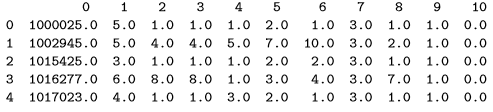
\includegraphics{Annotation 2020-03-23 185932.png}
\end{figure}
\subsubsection{Normalización.}
Aplicamos normnalización maxmin para mejorar el rendimiento y evistar que la columna con valores más altos monopolize el modelo. 
\begin{lstlisting}
names = df.columns[0:10]
scaler = MinMaxScaler() 
scaled_df = scaler.fit_transform(df.iloc[:,0:10]) 
scaled_df = pd.DataFrame(scaled_df, columns=names)
scaled_df[10]= df[10]
\end{lstlisting}
\subsubsection{Separar los datos.}
En este ejercicio separamos los datos en 2 sets, el de entrenamiento y el de test. Aprovechamos la versatilidad de la librería pandas para quitar la primera columna, pues el ID del paciento no influye en nada. Trasponemos los datos para que el finchero NeuralNetwork.py pueda trabajar con ellos.
\begin{lstlisting}
x=scaled_df.iloc[0:500,1:10].values.transpose()#500 para train
y=df.iloc[0:500,10:].values.transpose()
xval=scaled_df.iloc[501:683,1:10].values.transpose()
yval=df.iloc[501:683,10:].values.transpose()#168 para el tets
\end{lstlisting}
\subsection{Implementación de la red.}
En este apartado hacemos uso de las funciones del NeuralNetwork.py, la razón de desarrollar dicho fichero fue poder implementar redes neuronales de forma sencilla y poder aplicarla en distintos problemas sin tener que programar lo mismo otra vez. Ahora lo vemos en práctica.\\
Declaramos la red neuronal con los valores de entrenamiento y un learning rate de 0.01. La red funciona con una arquitectura [9 - 15 - 1], la cual utiliza funciones de salida lineales en la capa intermedia y una sigmoidal en la de salida. Utiliza como función de error, en lugar del clásico MSE, el Cross-Entropy. El algortimo de aprendizaje utilizado es el descenso por gradiente, el cual implementa el algoritmo de backpropagation.\\
Tanto la arquitectura como el learning rate son valores que hemos definido basandonos en la exoeriencia, en el anexo se muestran diversas implementaciones que nos han llevado a elegir la mejor.
\begin{lstlisting}
nn = NeuralNetwork(x,y,0.01,0)
nn.gradient_descent(50000)
\begin{figure}[H]
\centering
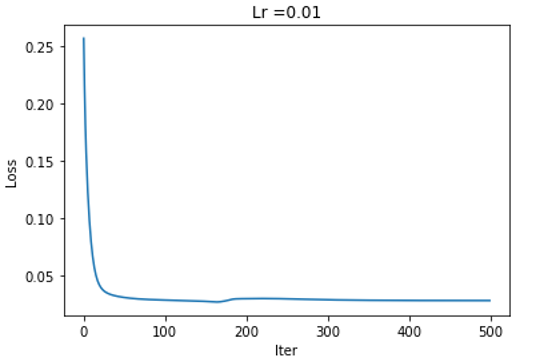
\includegraphics{Annotation 2020-03-23 190119.png}
\end{figure}
\end{lstlisting}
Imprimimos los resultados, nótese que este modelo no usa regularización.
\begin{lstlisting}
pred_train = nn.predict(x, y)
pred_test = nn.predict(xval, yval)
Acc: 0.9240000000000003
Acc: 0.9835164835164836
\end{lstlisting}
\subsubsection{Con regularización.}
Tras diversas pruebas, el valor 0.7 el que mejor rendimiento aporta. Elevando el acierto en el test al máximo.
\begin{lstlisting}
pred_train = nn.predict(x, y)
pred_test = nn.predict(xval, yval)
Acc: 0.9360000000000003
Acc: 1.0
\end{lstlisting}
\subsection{Visualización.}
Para visualizar los datos de dorma más explicativa se ha recurrido a una matriz de confunción que muestra el número de positivos clasificados correctamente, falsos positivos, falsos negativos, y  negativos clasificados correctamente. La función es la siguiente:
\begin{lstlisting}
def plotCf(a,b,t):
    cf =confusion_matrix(a,b)
    plt.imshow(cf,cmap=plt.cm.Blues,interpolation='nearest')
    plt.colorbar()
    plt.title(t)
    plt.xlabel('0         Predicted         1')
    plt.ylabel('1          Actual            0')
    tick_marks = np.arange(len(set(a))) # length of classes
    class_labels = ['0','1']
    plt.xticks(np.ndarray([0,1]))
    plt.yticks(np.ndarray([0,1]))
    for i,j in itertools.product(range(cf.shape[0]),range(cf.shape[1])):
        plt.text(j,i,format(cf[i,j],'d'),horizontalalignment='center',
           color='white' if cf[i,j] > (cf.max()*0.7) else 'black')
    plt.show();
\end{lstlisting}
Aquí podemos aplicar el threshold que deseamos, como estamos hablando de un tema tan sensible como el cancer, nuestro umbral debe ser alto para solo afirmar en caso de mucha certeza.

\begin{lstlisting}
nn.X,nn.Y=xval, yval 
target=np.around(np.squeeze(yval), decimals=0).astype(np.int)
predicted=np.around(np.squeeze(nn.predict(xval,yval)), decimals=0)
plotCf(target,predicted,'Cf Validation Set')
\end{lstlisting}
\begin{figure}[H]
\centering
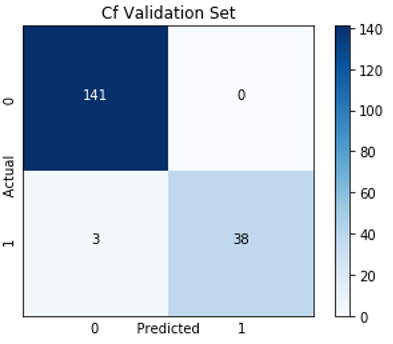
\includegraphics[scale=0.8]{Annotation 2020-03-23 190419}
\end{figure}
El modelo, incluso sin regularización, muestra un resultado excelente. Solo hemos clasificado 3 correos mal, todos eran spam y los hemos clasificado como correos ordinarios.

\subsection{Implementación con regresión logística.}
Con el fin de comprobar si un modelo más rápido y sencillo podría superar al ya explicado, hemos implementado regresión logística. Como era de esperar, la regresión logística no es suficiente para tratar problemas de esta embergadura.
\begin{figure}[H]
\centering
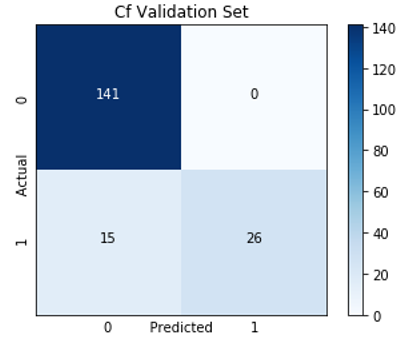
\includegraphics[scale=0.8]{Annotation 2020-03-23 193133.png}
\end{figure}
\newpage
\section{Ejercicio de clasificación de correo electrónico.}
Al igual que en la sección anterior, éste ejercicio implementa las funciones definidas en el archivo NeuralNetwork.py.\\ En este caso el ejercicio exige un enfoque ligeramente diferente respecto al anterior a causa de los datos. Los datos utilizados son numerosos mensajes, los cuales algunos son spam y otros mensakes corrientes. De dichos mensajes solo se pueden extraer sus palabras, así que en este caso, no tenemos distintas características que evaluar.
\subsection{Carga, comprensión y transformación de los datos.}
Como ya hemos dicho, el dataset está compuesto por frases y su correspondiente etiqueta, hay tres columnas vacías que quitamos.
\begin{lstlisting}
import pandas as pd
import numpy as np
import re
raw = pd.read_csv('spam.csv', delimiter = ',')
raw.head()
\end{lstlisting}
\begin{figure}[H]
\centering
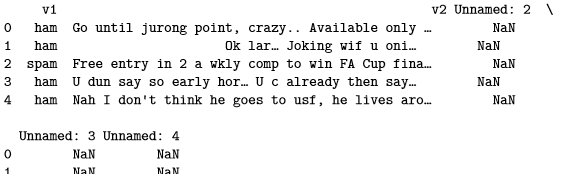
\includegraphics[scale=0.9]{Annotation 2020-03-23 174228.png}
\end{figure}
\begin{lstlisting}
raw.drop(['Unnamed: 2' ,'Unnamed: 3' ,'Unnamed: 4'], axis=1)
raw = raw.dropna(how='any',axis=0)# drop Nan rows
raw.head()
\end{lstlisting}
\begin{figure}[H]
\centering
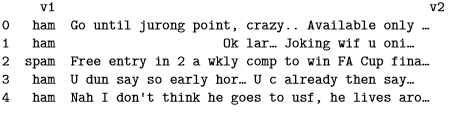
\includegraphics{Annotation 2020-03-23 174341.png}
\end{figure}
Como ya hemos comentado, la única información que podemos extraer de los datos son palabras, en total hay aproximadamente 1000. Como no es viable desarrollar en nuestro equipo una red neuronal con 10000 valores en la capa de entrada, debemos sesgar cuáles queremos.\\ En este caso hemos elegido 100, las 100 que más se repiten. Nótese que con intención de hacer un modelo más eficiente, se podrían considerar otros criterios a parte de la frecuencia de aparición en el dataset.\\
Contamos las palabras:
\begin{lstlisting}
columns=[] 
rows = [] 
y = list(raw.v1)#lo usaremos luego 
for i in range (0,len(raw.v2)): 
    try:
         rows.append(re.sub("[^\w]", " ", raw.v2[i]).lower().split()) 
         columns = columns + re.sub("[^\w]", " ", raw.v2[i]).lower()
    except: 
        print('Error in:' ,raw.v2[i])
from collections import Counter 
    counts = Counter(columns)

    print(counts)
\end{lstlisting}
\begin{figure}[H]
\centering
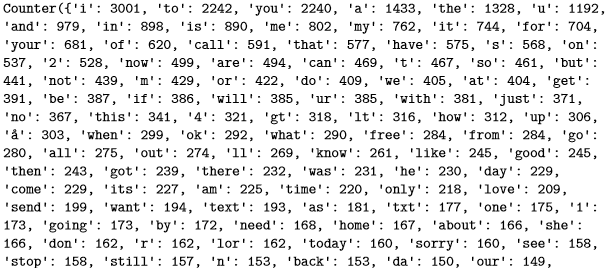
\includegraphics[scale=0.83]{Annotation 2020-03-23 182424.png}
\end{figure}
Elegimos las palabras:
\begin{lstlisting}
columns = list(dict.fromkeys(columns))#delete repeated values 
counts_list = [key for key, _ in counts.most_common()] 
df_columns = counts_list[0:100] 
df_columns.append('y') 
print(df_columns)
\end{lstlisting}
\subsubsection{Transformar la información.}
Ahora lo relevante es determinar cómo vamos a introducir la infromación en la red. Las redes neuronales no aceptan otra entrada que no sea de caracter numérico, eso nos lleva a transformar nuestro set de datos, utilizaremos un 1 cuando la palabra de la frase sea una de las palabras elegidas como entrada dee la red y utilizaremos un 0.
\begin{lstlisting}
binary_rows = np.zeros((len(rows),len(df_columns)),dtype=int) 
for i in range(0, len(rows)): 
    for k in range(0,len(rows[i])):
        if rows[i][k] in df_columns: 
	    binary_rows[i][df_columns.index(rows[i][k])]=1
         if k == (len(rows[i])-1) and y[i]=='spam':#if spam=>1 
            binary_rows[i][100]=1
print(binary_rows[2])
\end{lstlisting}
\begin{figure}[H]
\centering
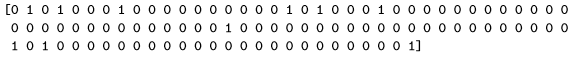
\includegraphics[scale=0.83]{Annotation 2020-03-23 182035.png}
\end{figure}
Creamos un dataframe nuevo con las frases cargadas como secuencias binarias.
\begin{lstlisting}
dataframe = pd.DataFrame(binary_rows,columns=df_columns) 
dataframe.head(5)
\end{lstlisting}
\begin{figure}[H]
\centering
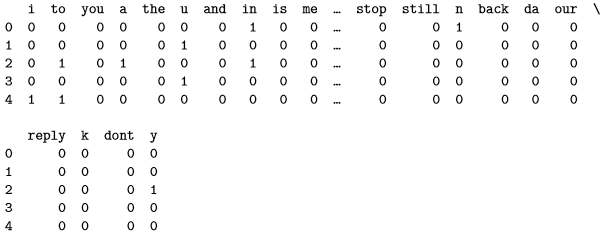
\includegraphics[scale=0.83]{Annotation 2020-03-23 182154.png}
\end{figure}
Por último, creamos los datos en listas para imputarlos porteriormente en la red.
\begin{lstlisting}
Y = (dataframe.y).to_numpy() 
dataframe.drop(['y'], axis=1, inplace=True)
X = dataframe.to_numpy().T 
size = int(X.shape[1] * 0.70) 
x_train, x_test = X[:,0:size], X[:,size:] 
y_train, y_test = Y[0:size], Y[size:]
\end{lstlisting}
\subsection{Implementación de la red.}
De nuevo utilizamos el fichero NeuralNetwork.py, en este caso, la  arquitectura  que mejor rendimiento muestra es la 100-25-1, 25 neuronas en una única capa oculta y un ratio de aprendizaje (learning rate) de 0.2. Diversas arquitecturas puede contrastarse en el anexo de este trabajo.
\begin{lstlisting}
from NeuralNetwork import * 
nn = NeuralNetwork(x_train,y_train,0.02,[100,25,1],0)
nn.gradient_descent(5000)#gradient descent algorithm
\end{lstlisting}
\begin{figure}[H]
	\centering
	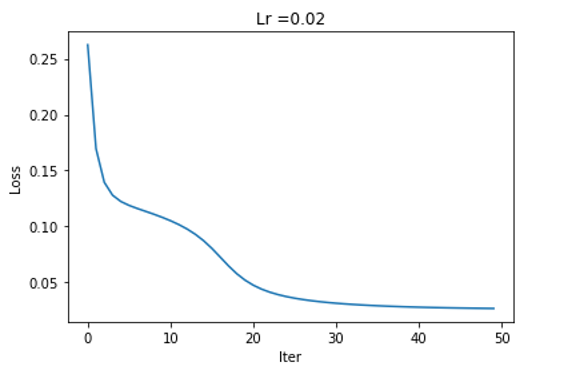
\includegraphics[width=12.0cm,height=8.5cm]{Annotation 2020-03-23171823}
\end{figure}
\subsection{Visualización.}
Implemantamos de nuevo la función de la matriz de confunción. La función es la siguiente:
\begin{lstlisting}
def plotCf(a,b,t):
    cf =confusion_matrix(a,b)
    plt.imshow(cf,cmap=plt.cm.Blues,interpolation='nearest')
    plt.colorbar()
    plt.title(t)
    plt.xlabel('0         Predicted         1')
    plt.ylabel('1          Actual            0')
    tick_marks = np.arange(len(set(a))) # length of classes
    class_labels = ['0','1']
    plt.xticks(np.ndarray([0,1]))
    plt.yticks(np.ndarray([0,1]))
    for i,j in itertools.product(range(cf.shape[0]),range(cf.shape[1])):
        plt.text(j,i,format(cf[i,j],'d'),horizontalalignment='center',    
	   color='white' if cf[i,j] > (cf.max()*0.7) else 'black')
    plt.show();
\end{lstlisting}
Llamamos de nuevo a la función. Observamos que esta vez el rendimiento está al rededor del 95 por ciento.
\begin{lstlisting}
nn.X,nn.Y=x_test, y_test 
target= nn.Y
predicted=nn.predict(x_test,y_test) 
plotCf(target,predicted[0],'Cf Validation Set')
\end{lstlisting}
\begin{figure}[H]
\centering
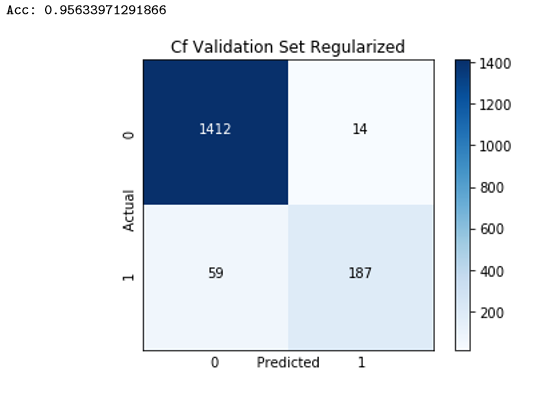
\includegraphics[width=12.0cm, height=8.5cm]{Annotation 2020-03-23 161410}
\end{figure}
Hemos fallado 63 mensajes, de los cuales, 14 han sido clasificado erroneamente como spam y 59 como spam
\subsubsection{Con regularización.}
En este caso la regularización no aporta nada, este método ha sido evaluado con distintos valores pero ninguna prueba ha aportado ninguna mejora. Teniendo en cuenta esto, es posible que el anterior resultado sea el correspondiente al alcanzar el mínimo absoluto en la función de error.

\subsection{Implementación con regresión logística.}
Como podemos observar, en este caso la regresión logística es igual de efectiva que la red neuronal, esto es otra indicación que podemos haber hayado el mínimo absoluto de la función de error.
\begin{lstlisting}
logistic_regression= LogisticRegression()
logistic_regression.fit(x_train.T,y_train)
threshold = 0.5
y_pred = np.where(logistic_regression.predict_proba(x_train.T)[:,1]
					 > threshold, 1, 0)
plotCf(target,y_pred,'Cf Validation Set Logistic Regression')
\end{lstlisting}
\begin{figure}[H]
\centering
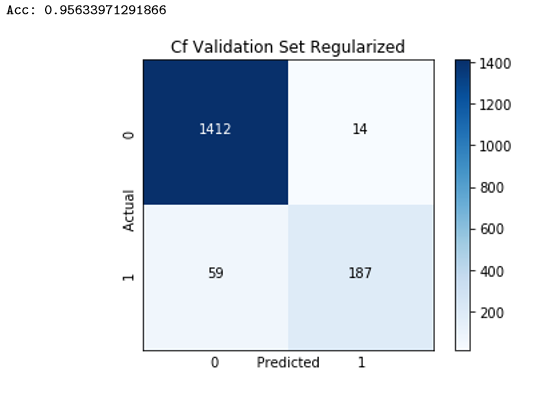
\includegraphics[width=12.0cm, height=8.5cm]{Annotation 2020-03-23 161410}
\end{figure}
\newpage
\section{Visión Artificial.}
La visión humana es un sistema muy complejo y poderoso. Simplemente
visualizando una fotografía, el sistema visual humano es capaz
de percibir y deducir una gran cantidad de información acerca de ella. Por ejemplo, con la fotografía mostrada, podemos interpretar una inmensa varideda de tonos y colores deducidos del efecto de la luz incidiendo en los pétalos de la flor.
Gracias al proceso de detección que realiza el ojo humano, podemos reconocer figuras, bordes, contornos, etc., podemos incluso segmentar la foto del resto dela imagen e interpretar factores como la profundidad a pesar de estar viendo una imágen en dos dimensiones (virtualmente).\\
El proceso seguido para ello consta de dos partes. Por un lado, la luz reflejada por los objetos
atraviesa llega hasta nuestos ojos, formándose en la retina una imagen invertida en dos
dimensiones.  Por otro lado, dicha imagen estransformada en impulsos nervisoso y trasladada a la parte posterior de cerebro, 
el cual reconstruye un modelo en tres dimensiones de la imagen, gracias a la intervención de millones de neuronas. 
Al mismo tiempo nuestro cerebro asocia la imagen con el concepto previamente asimilado de lo que es de una flor y la reconoce como tal.
\begin{figure}[H]
\centering
\includegraphics[width=8.5cm, height=5.35cm]{flor.jpg}
\end{figure}
\noindent
La Visión Artificial, conocida también como visión por computador, es la disciplina que trata de otorgar a los ordenadores la capacidad de percibir, procesar  e interpretar imágenes de forma análoga a la visión humana. Nótese que el ordenador percibe imágenes como matrices de valores numéricos, típicamente comprendidos en el rango de 0 a 255. En el caso de las imágenes RGB este rango se mantiene pero se amplia la cantidad de información a tres matrices, una por color.\\
En las siguientes subsecciones veremos las aplicaciones más comunes de la visión artificial, además de explicar sus limitaciones.
\subsection{Aplicaciones.}
En la actualidad existe una gran variedad de aplicaciones de la visión artificial, es una ciencia que está presente en muchísimos campos. Los más comunes son:
\begin{itemize}
\item Reconocimiento óptico de carácteres (OCR): esta técnica consiste en la lectura e identificación de los carácteres alfanuméricos de una imagen. A día de hoy está considerado un problema sencillo de resolver. Su primera aplicación data de los años 60, y fue empleado en el reconocimiento de códigos postales por el servicio de correo de Estados Unidos.
\item Construcción de modelos 3D (fotogrametría). esta técnica se basa en la construcción de figuras 3D mediante imágenes 2D.
\item Medicina: la medicina es uno de los campos que más partido saca de la visión artificial. Un ejemplo es la detección automática de melanomas.
\item Monitorización:
\end{itemize}
\newpage
\section{Redes convolucionales.}
En este apartado explicaremos las redes neuronales que vamos a necesitar para implementar el último ejercicio del trabajo; estas son las redes convolucionales, en adelante CNN. Las CNN se utilizan en problemas de clasificación de imágenes como alternativa al tipo de red que ya hemos visto, pues este queda absoleto ante una gran cantidad de datos en la capa de entrada, como es en el caso de las imágenes.\\ Procedemos a explicar las novedades y conceptos que dicha red incorpora.\\

\subsection{Filtros.}
Los filtros son matrices de tamaño configurable, siempre menores que la matriz de entrada, estos se aplican por toda la imagen. El resultado es una nueva matriz cuyos datos derivan de los productos matriciales del filtro y la fotografía. Estos filtros son capaces de extraer características como líneas, curvas, contronos, etc.  \\Es decir, si aplicamos un filtro para las líneas verticales y otro para las horizontales, el resultado serán dos imágenes, cada una solo con la información para la que hemos aplicado el filtro.
\begin{figure}[H]
\centering
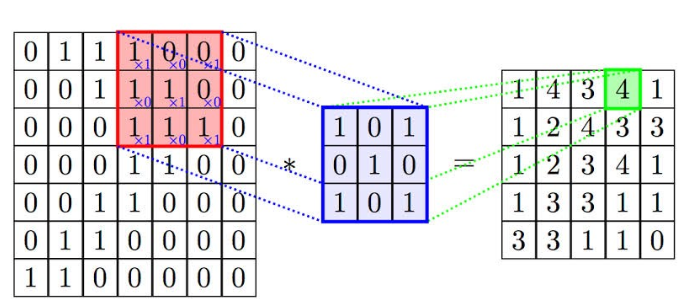
\includegraphics[width=12.0cm, height=4.5cm]{Annotation 2020-04-13 191448.png}
\end{figure}
Hay tres parámetros imprescindibles a la hora de definir un filtro:
\begin{itemize}
\item Tamaño: podemos definir el tamaño del filtro, que varía en función del tamaño de la imagen y de las características que nos gustaría extraer.  Normalmente se utilizan matrices. cuadradas
\item Stride:  es el intervalo de posiciones en el que aplicamos el filtro. Si nuestro filtro tiene un stride de 1, el filtro se desplazará por la imagen de píxel en píxel,  si ponemos el valor a dos, lo hará de dos píxeles en dos píxeles. Es decir, se aplicará el filtro cubriendo todos los valores de la imagen, pero el centro del filtro solo coincidirá con la mitad los datos de la imagen. 
\item Padding: es evidente que al aplicar un filtro no es posible que este recorra la matriz de forma equitativa independientemente del stride. Por ejemplo, en caso de los datos de las esquinas solo se les aplicaría una vez según la explicación dada. El padding indica un margen adicional que introducimos con valores de cero alrededor de la matriz para permitir aplicar el filtro por la totalidad de la imagen. \\Existen dos tipos de padding:
	\begin{itemize}
	\item Valid: implica que no hay padding, lo que hace que se pierda información de los contornos de la imagen.\begin{figure}[H]
\centering
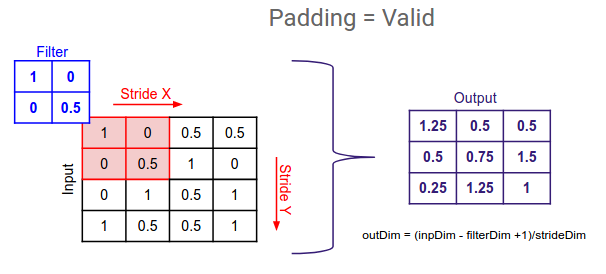
\includegraphics[width=10.0cm, height=4.5cm]{Annotation 2020-04-13 214927.png}
\end{figure}
	\item Same: incluye tantas como sea necesario para que el tamaño de la salida sea igual al de entrada.\begin{figure}[H]
\centering
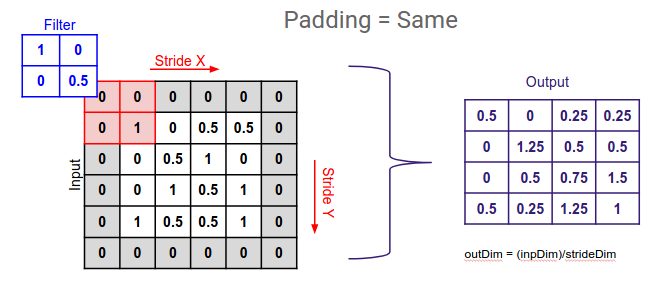
\includegraphics[width=11.0cm, height=4.5cm]{Annotation 2020-04-13 215118.png}
\end{figure}
	\end{itemize}
\end{itemize}
Estos factores son los que determinan el tamaño de la matriz de salida (n), siendo el tamaño del filtro (f), el de la matriz de entrada (i), padding (p) y stride(s).
\[
n=\frac{i+2p-f}{s}  +1
\]


\subsection{Capa convolucional.}
Las capas convolucionales son el núcleo de las CNN, son las capas de la arquitectura donde se aplica la operación de convolución. La operación consiste en desplazar el filtro por la matriz, aplicándolo en cada dato hasta cubrirla completamente. En cada desplazamiento se realiza un producto matricial. Dicho proceso se repite tantas veces como números de filtros hayamos dispuesto en nuestra capa convolucional (k), de forma que si hemos dispuesto 32 filtros para una imagen de 28*28 píxeles, la salida será de 28*28*32 = 25.088 píxeles.
 \\La siguente fórmula muestra cómo se calcula el número de datos correspondiente a la salida de la capa convolucional.

\[
n=\frac{i+2p-f}{s}  +1
\]
\[
output = k * n
\]
A primera vista puede parecer que 25.088 datos para una foto tan simple resulta algo disparatado, pero si nos planteamos la cantidad de datos que habría en una red neuronal convencional, no lo es. Supongamos que tenemos la misma imagen, pero en lugar de una capa convolucional, implementamos una capa con el mismo número de neuronas que el de la capa de entrada. Si cada entrada está conectada a todas las neuronas de la capa siguiente (característica bastante frecuente), el resultado del número de datos sería el cuadrado de la entrada, es decir, 614.656 datos, solo para abordar los pesos. \\
Aún con esta ventaja, las CNN cuentan con otro mecanismo para aligerar la carga de información.
\subsection{La capa de pooling.}
Esta es la capa que se encarga de realizar la reducción del volumen de datos, perdiendo la menor información posible. Supongamos que tenemos el mismo bloque de datos del ejemplo anterior, 25.088 datos en una matriz de 28*28*32. Es evidente que si queremos reducir la dimensionalidad de la matriz, no podemos alterar la dimension de 32, pues estaríamos quitando filtros que se han añadido en la capa convolucional.\\
Existen dos tipos de pooling:
\begin{itemize}
\item Max pooling: consiste en reducir las dimensiones de una matriz, separándola en subconjuntos de tamaño configurable y conservando solo el valor mayor de cada fragmento. Dichos subconjuntos se hacen siguendo el mismo criterio que seguimos para desplazar los filtros, de forma que, a mayor stride, más se reducirá la matriz.
\begin{figure}[H]
\centering
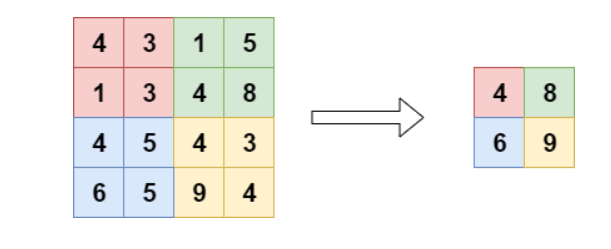
\includegraphics[width=11.0cm, height=4.5cm]{maxpool.png}
\end{figure}
\item Mean pooling: el proceso es análogo al maxpooling, solo que en esta ocasión, el valor conservado es el medio de los subconjuntos.
\begin{figure}[H]
\centering
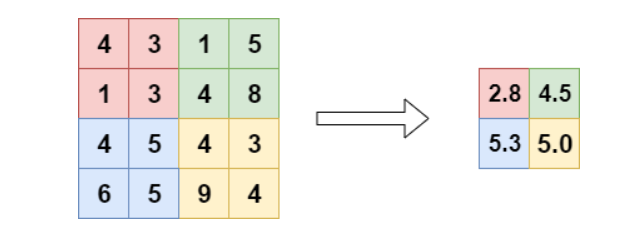
\includegraphics[width=11.0cm, height=4.5cm]{meanpool.png}
\end{figure}
\end{itemize}
\subsection{Fully connected layer y red neuronal.}
Esta capa, también conocida como flatten, es una capa a la que se conectan a todas las salidas de la capa anterior (convolucional o de pooling) con una capa con tantas neuronas como datos. Posteriormente se realiza una arquitectura con una o dos capas intermedias y una capa de salida con tantas neuronas como clases tenga nuestro problema de clasificación. En estas capas puede aplicarse regularización.
\subsection{Arquitecturas.}
En el desarrollo de la CNN, podemos usar nuestros conocimientos teóricos para programar, pero existen ciertas redes muy conocidas que han demostrado en numerosos problemas un buen rendimiento. En la práctica intentaremos imitar la arquitectura de dichas redes.
\begin{itemize}
\item LeNet: es una red neuronal desarrollada por Yann LeCun en 1998. Su versión más conocida es la arquitectura con cinco capas. \begin{figure}[H]
\centering
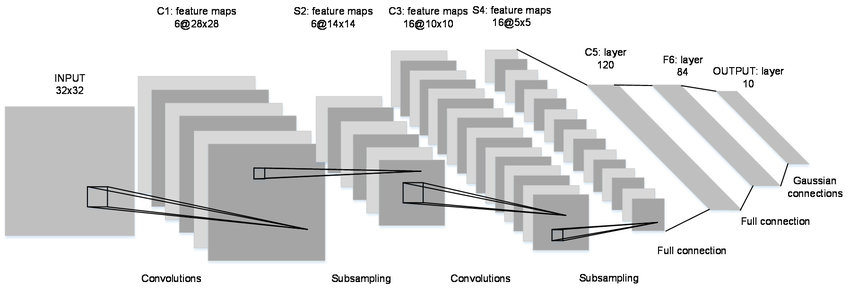
\includegraphics[width=14.0cm, height=4.5cm]{lenet5.png}
\end{figure}
\item AlexNet: desarrollada por Alex Krizhevsky, ganó el concurso ImageNet Large Scale Visual Recognition Challenge en septiembre de 2012. Es una red neuronal muy eficiente pero que conlleva un alto coste computacional debido a su parelilización en dos CNN , es inviable usarla sin GPU.\begin{figure}[H]
\centering
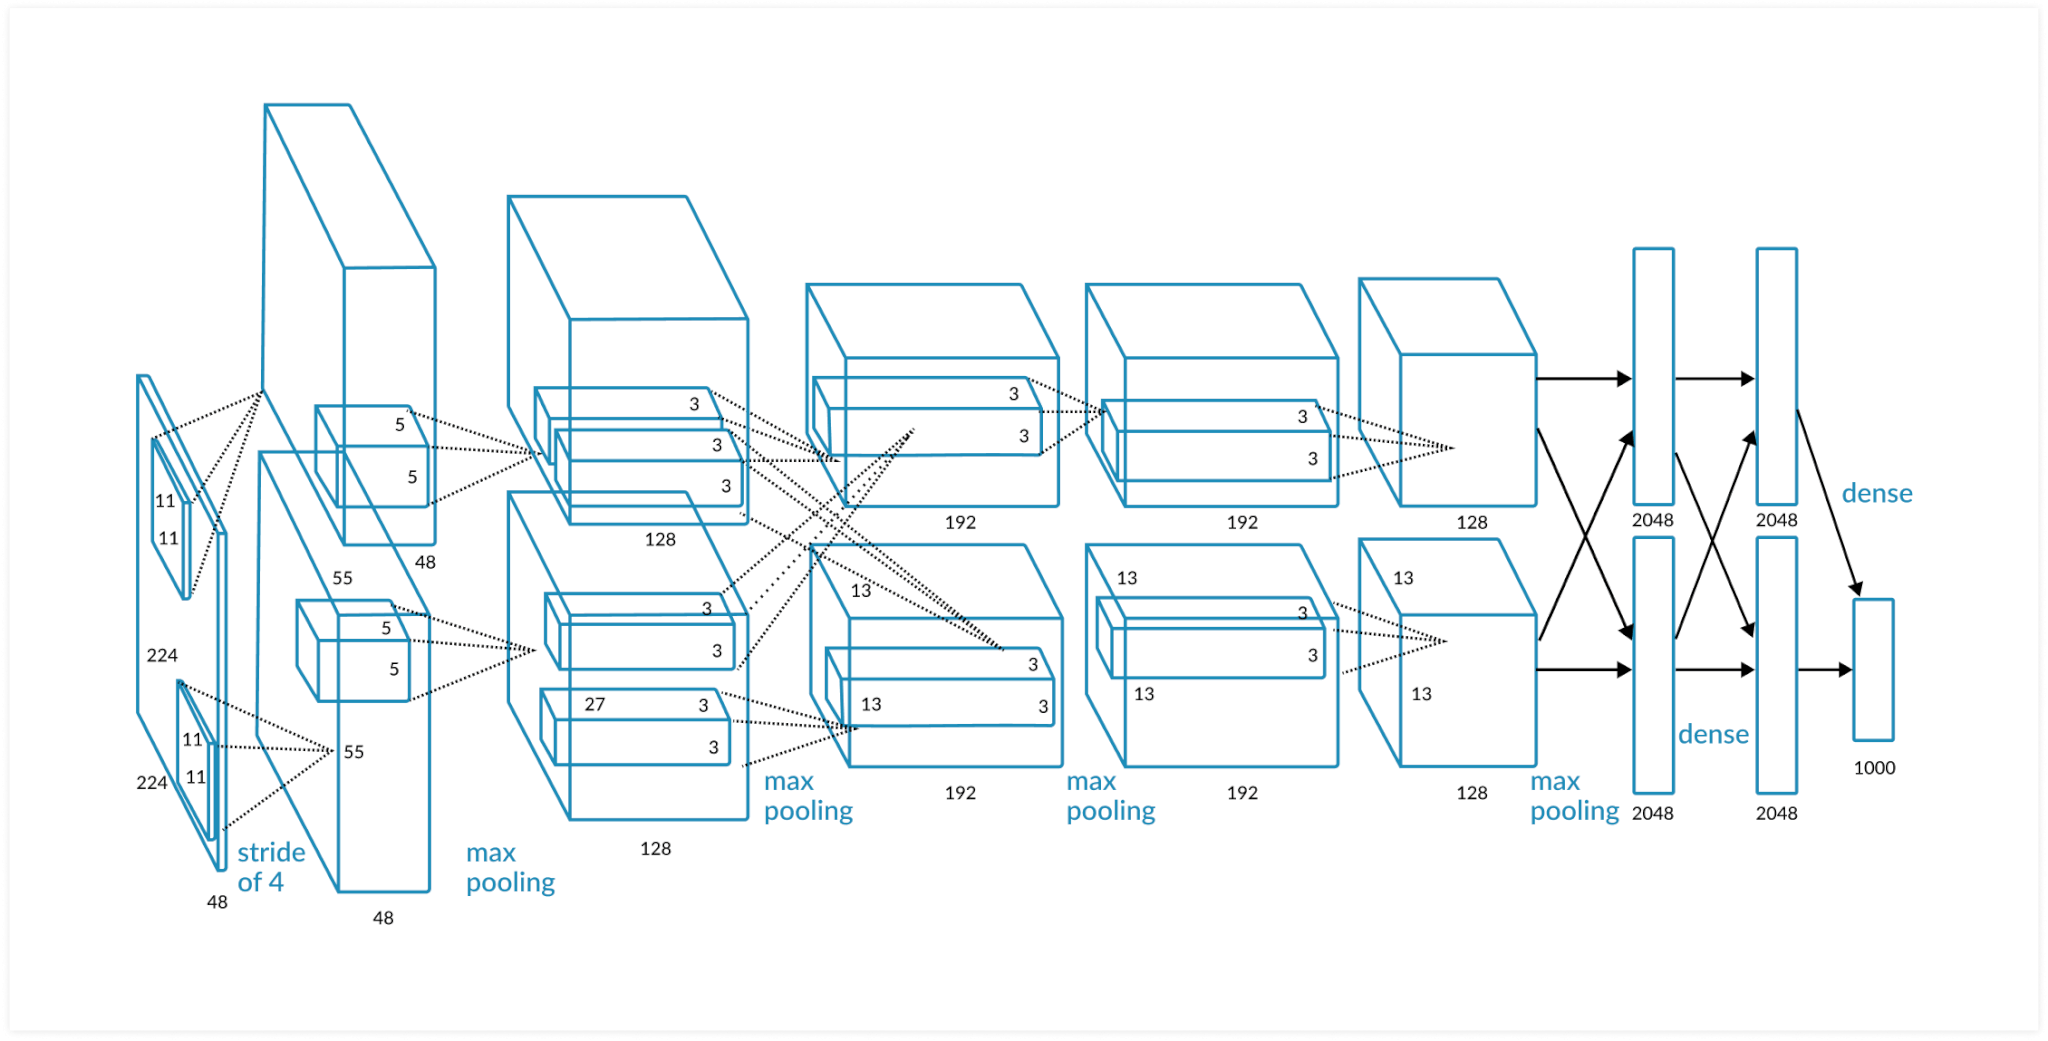
\includegraphics[width=14.0cm, height=4.5cm]{AlexNet2012.png}
\end{figure}
\item VGG16: propuesta por K. Simonyan y A. Zisserman. El modelo alcanzó un 0.927 de precisión en ImageNet, un dataset de 14 milliones de imagenes en 1000 classes. \begin{figure}[H]
\centering
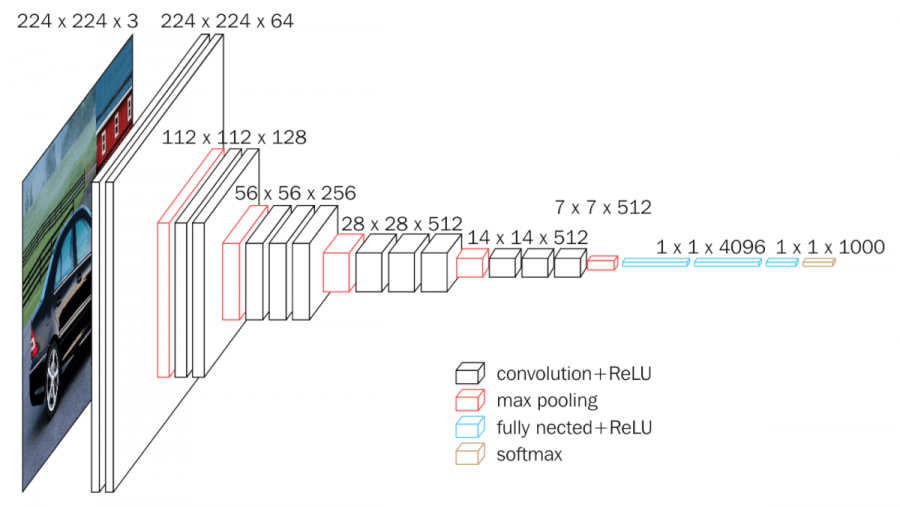
\includegraphics[width=12.0cm, height=4.5cm]{vgg16-1-e1542731207177.png}
\end{figure} 	
\item ResNet: desarrollada por Microsoft en 2015, también ganó el ImageNet Large Scale Visual Recognition Challenge. Tiene varias configuraciones: con 50, 101 y 152 capas.\begin{figure}[H]
\centering
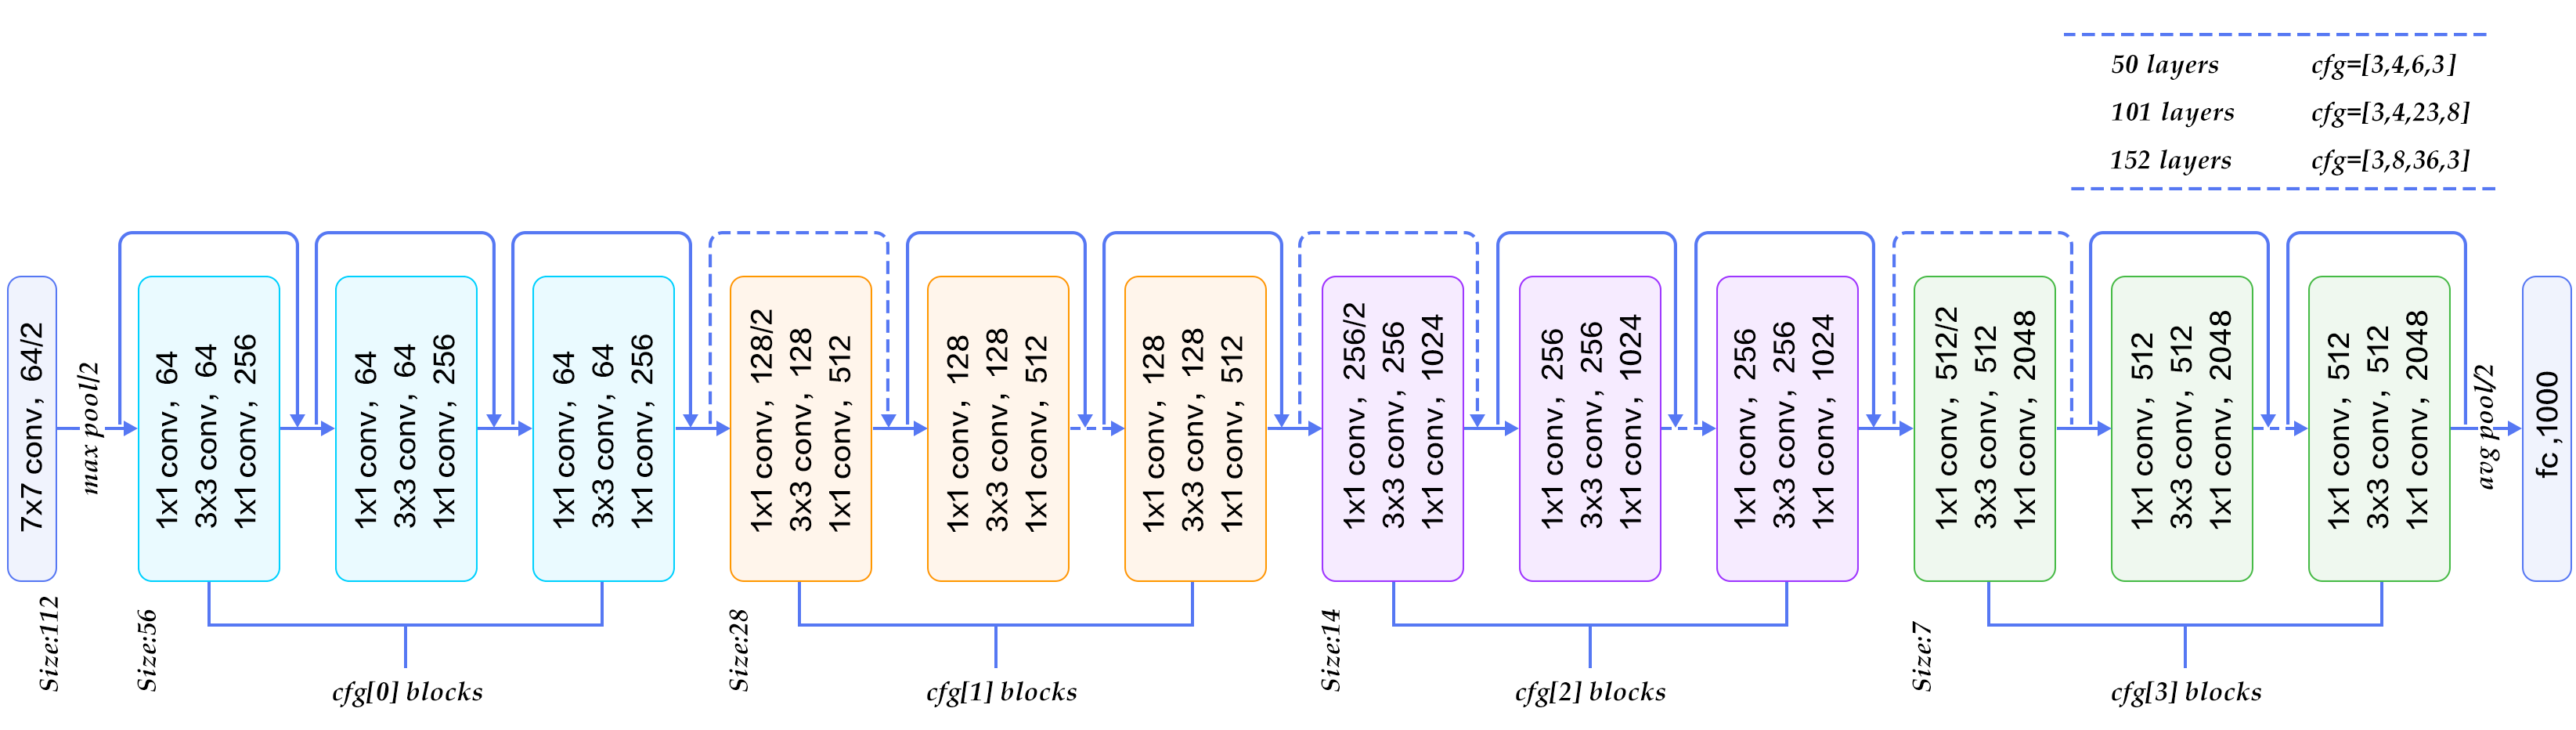
\includegraphics[width=12.0cm, height=4.5cm]{resnet.png}
\end{figure} 	
\end{itemize}

\newpage

\section{Aplicación práctica: Clasificación de señales de tráfico.}
En el siguiente ejercicio vamos a clasificar 43 tipos de imágenes de señales de tráfico en python mediante una CNN. \\
El set de datos que utilizaremos contiene 32902 imágenes divididas en carpetas en función del tipo para el entrenamiento y 12630 para el test.
\subsection{Carga de los datos.}
En esta ocasión los datos de entrenamiento y test están almacenados de distinta forma, por ello es necesario que implementemos dos funciones para realizar la carga.
\subsubsection{Carga de datos de entrenamiento.}
Los datos de entrenamiento están almacenados dentro en 43 carpetas detro de la carpeta "Train". Debemos recorrer dicho directorio, importar las imágenes RGB y transformarlas en un array de cara a poder manejarlas posteriormente. Como no todas las fotos presentan el mismo tamaño, modificamos ligeramente sus dimensiones con el fin de trabajar siempre con matrices del mismo tamaño, en este caso de 30*30.\\
Determinaremos la clase de cada imagen en el momento de carga basandonos en la carpeta en la que se encuentre. Una vez relizada la carga, devolvemos las imégenes y su clase en formato de matriz.
\begin{lstlisting}
def load_train(folders,size):
    X=[]
    Y=[]
    for i in range(folders) :
        path = "ruta al directorio principal"
        folder=os.listdir(path)
        for img in folder:
            try:
                image=cv2.imread(path+img)
                image_RGB = Image.fromarray(image, 'RGB')
                resized_image = image_RGB.resize(size)
                X.append(np.array(resized_image))
                Y.append(i)
            except AttributeError:
                print("Error loading picture ", img)
    return np.asarray(X),np.asarray(Y)
\end{lstlisting}
\subsubsection{Carga de datos de prueba.}
Esta función carga los datos de prueba. A diferencia de en el apartado anterior, la clase de cada foto se extrae de un archivo csv de con los metadatos. En el resto de la función es como igual a la utilizada en la carga de datos.

\begin{lstlisting}
def load_train(folders,size):
    X=[]
    Y=[]
    for i in range(folders) :
        path = "ruta al directorio principal"
        folder=os.listdir(path)
        for img in folder:
            try:
                image=cv2.imread(path+img)
                image_RGB = Image.fromarray(image, 'RGB')
                resized_image = image_RGB.resize(size)
                X.append(np.array(resized_image))
                Y.append(i)
            except AttributeError:
                print("Error loading picture ", img)
    return np.asarray(X),np.asarray(Y)
\end{lstlisting}
\subsection{Manipulación de los datos.}
Tras cargar los datos debemos mezclar los datos. El modelo debe tener las imágenes barajadas para no ir entrenando clase por clase, esto afecta drásticamente al rendimiento. \\
Tambíen creamos un set de datos de validación del 20\% del volumen total de entrenamiento para estudiar la evolución del entrenamiento en tiempo real.
\begin{lstlisting}
X,Y=load_train(43,[30,30])
#shuffle the data
s=np.arange(X.shape[0])
np.random.seed(43)
np.random.shuffle(s)
X=X[s]
Y=Y[s]
#Spliting the images 
(X_train,X_val)=X[(int)(0.2*len(Y)):],X[:(int)(0.2*len(Y))]
X_train = X_train.astype('float32')/255 #Train normalization 
X_val = X_val.astype('float32')/255 #Test normalization
(y_train,y_val)=Y[(int)(0.2*len(Y)):],Y[:(int)(0.2*len(Y))]
\end{lstlisting}
\subsection{Arquitectura.}
La arquitectura escogida es una versión simplificada que al modelo VGG16. La arquitectura es la siguiente.
\begin{itemize}
\item Capa convolucional: 32 filtros de tamaño 5*5, stride de 1 y valid para el padding.
\item Capa convolucional: 64 filtros de tamaño 3*3, stride de 1 y valid para el padding.
\item Capa maxpooling: tamño de 2,2 con stride de 1 y valid para el padding.
\item Capa de dropout del 25\%: descartamos el 25\% de los datos aleatoriamente para prevenir overfitting.
\item Capa convolucional: 64 filtros de tamaño 3*3, stride de 1 y valid para el padding.
\item Capa maxpooling: tamaño de 2,2 con stride de 1 y valid para el padding.
\item Capa de dropout del 25\%.
\item Capa fully-connected.
\item Capa de 256 neuronas.
\item Capa de dropout del 50\%.
\item Capa de salida, 43 neuronas con la función softmax.
\end{itemize}
Los elementos de la arquitectura han sido elegidos como resultado del estudio de la materia mostrada y se han ido ajustando en función de los resultados obtenidos durante el derrallo. Las principales razones son:
\begin{itemize}
\item Debido al tamaño de las fotos los filtros no sobrepasan el tamaño de 5. 
\item Dado que en todas las fotografías las señales no se ajustan a los bordes, los píxeles que forman el controno de la imagen no aportan información respecto a la naturaleza de la señal, es por ello que hemos decidido establecer el padding como valid.
\item Por otro lado, la razón de que el stride sea igual a 1, lo cual supone una bajada de rendimiento como se muestra en la fórmula del apartado X, es que no queremos perder información de imágenes con tan poca cantidad de píxeles.
\end{itemize}
\subsection{Entrenamiento y resultados.}
Por último, entrenamos la CNN utilizando el optimizador adam y el errore de crross-entropy, durante 5 iteraciones.
\begin{lstlisting}
#Compilation of the model
model=build_model()
model.compile(
    loss='categorical_crossentropy', 
    optimizer='adam', 
    metrics=['accuracy']
)
#entrenamos el modelo 55 iteraciones
epochs = 5
history=model.fit(X_train, y_train, batch_size=32, epochs=epochs,
				validation_data=(X_val, y_val))
\end{lstlisting}
\begin{figure}[H]
\centering
\includegraphics[width=6.0cm, height=4.5cm]{Annotation 2020-04-24 115814.png}
\end{figure}
\begin{figure}[H]
\centering
\includegraphics[width=6.0cm, height=4.5cm]{Annotation 2020-04-24 120025.png}
\end{figure}
\noindent
Vemos que la red funciona de forma correcta, con una rápida convergencia de la función de error. Como resultado en el set de prueba, obtenemeos una precisión del 96\%.

\begin{lstlisting}
X_test,Y_test=load_test([30,30])
X_test = X_test.astype('float32')/255 
y_pred = model.predict_classes(X_test)

from sklearn.metrics import accuracy_score
print(accuracy_score(Y_test, y_pred))
0.9691211401425178#casi un 97%
\end{lstlisting}

\end{document}	



